\section{Python Problem - AR System Identification}\label{sec:p6}

The signal is approximated using LMS algorithm. To find the best $L$, the script runs through multiple $L$'s and choose the one with the lowest MSE. The script also has regularization to avoid divergence, where $\lambda$ is selected among $\{1, 1^{-1}, ..., 1^{-9}\}$ by the lowest MSE. The result is showed in Figure \ref{fig:p6}, where the optimal setting is $L=1$ giving $w \approx 0.9514$ and $MSE \approx 0.0540$

\begin{figure}[htbp]
	\centering
	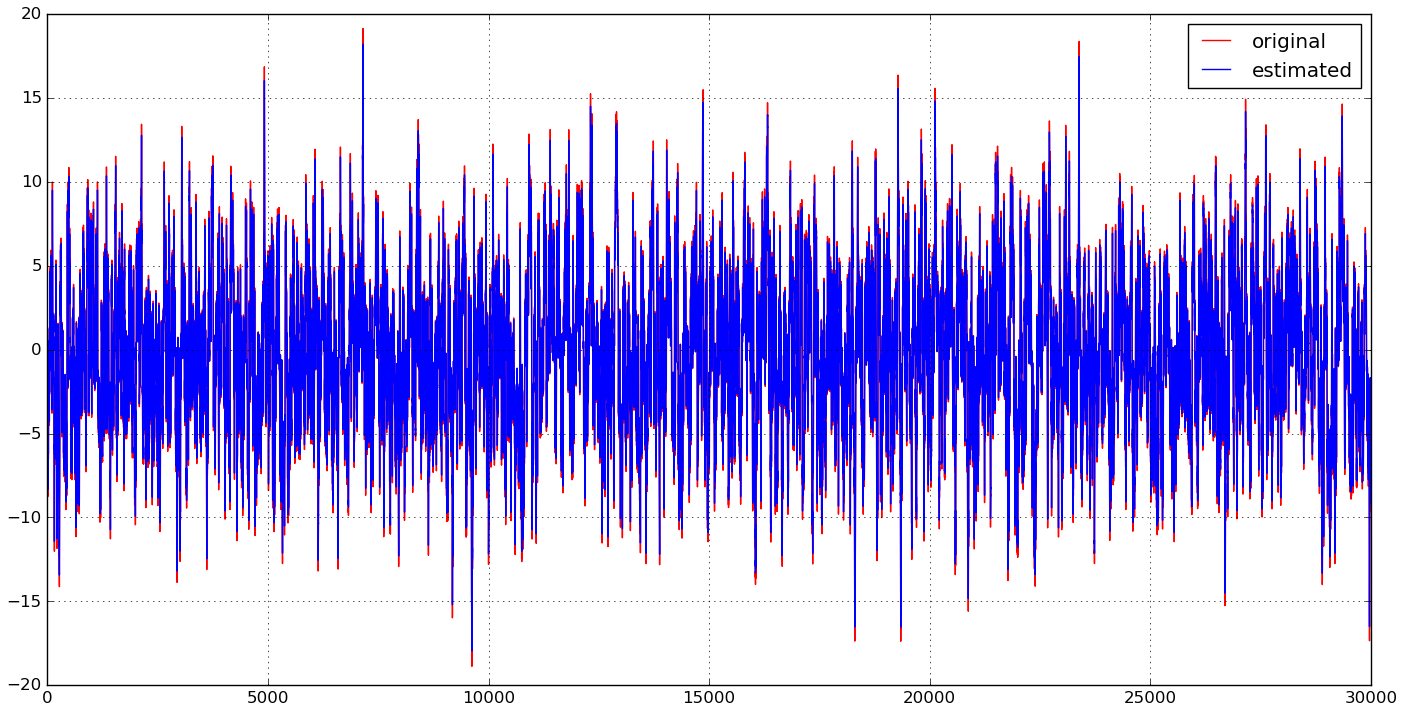
\includegraphics[width=\textwidth]{images/p6}
	\caption{Best LMS result with $L=1, w \approx 0.9514$, and $MSE \approx 0.0540$.}
	\label{fig:p6}
\end{figure}